\begin{ecpc}
 \chapter{Self- and ion-induced polarization in ethylene and propylene carbonate}
 \hyperlink{toc}{Return to TOC} 
  \section{\label{ch4:sec0:level1}Preface}
   
   Disclaimer: this chapter is subject to additional changes as it is not yet published.
   
   In this section I explore what effect an accurate treatment of polarizability has in simulations of liquid ethylene and propylene carbonate versus 
   the gas phase. Previous solvation thermodynamic work by Arslanargin et al. hypothesized that their results could be improved with a more physical
   treatment of polarization\cite{ayse2016ecpc}. This is because in a tetrahedrally coordinated complex with either of these solvents, each of the
   dipoles points in towards the ion, producing an effective repulsive interaction that the classical force field failed to capture. I begin with an
   examination of self-polarization which is an important effect in water, for example, where the dipole moment increases from $\sim$ 1.85 D in the 
   gas phase to somewhere between 2.3 -- 2.9 D. I find in both of these solvents the average dipole moment increase about 34\% over the gas phase 
   monomer sampled at the same temperature. Following this, I address the change of the dipole moment in molecules solvating a single Li\sur{+}.
   Unlike water where the dipole moment tends back towards the bulk value with increasing coordination number, the dipole moments of ethylene and
   propylene carbonate increase to just over 50\% greater than the gas phase average. The classical model using charges that reproduce bulk properties
   of each of these solvents underestimates the polarization effect, while re-fitted parameters to the ion/solvent dimer lead to an overestimation
   of the effect. I also examine interaction energies computed with the density functional flavor of SAPT between the \emph{ab initio} and classically
   generated trajectories. These results indicate that Li\sur{+} likely binds ethylene carbonate more tightly than propylene carbonate, though there
   remains no consensus on this in the literature. The coordination number is determined from the integral of the first peak in the ion/solvent 
   radial distribution function. Comparison to the literature indicates that my predicted coordination number of 3.8 in ethylene carbonate and 3.98
   in propylene carbonate are consistent with previous simulation results. However, these pretty uniformly underestimate the figure versus experimental
   methods. Since this is still a work in progress, some additional calculations and analysis steps are briefly discussed.
   
   This section addresses three of the questions I posed in Chapter \ref{ch1:sec6:level1},

   \begin{itemize}
       \item What sort of interactions? 
       \item How strong are they relative to one another?
       \item Do we need electronic structure theory to solve everything?
   \end{itemize}
  
  \section{\label{ch4:sec1:level1}Computational methods}
   \subsection{\label{ch4:sec1:level2}Initial configurations}
    Separate cubic boxes of 32 ethylene and propylene carbonate molecules were constructed and equilibrated in the NPT ensemble using Gromacs 4.6.7\cite{gromacs}.
    The molecules were modeled with the general Amber force field (GAFF). Simulations were propagated for 4 ns with configurations saved every 10
    steps to monitor solvent densities. Each simulation was performed at 310 K and 1 atm pressure. Velocity-rescaling and the Berendsen barostat
    were used to control temperature and pressure fluctuations, respectively. Final configurations were used as starting points for optimization at
    the density functional level.

    Single molecule and the previously described 32-molecule cells were optimized with CP2K 2.6.1\cite{hutter2014cp2k} at the PBE/DZVP-MOLOPT-SR-GTH
    level\cite{goedecker1996separable,perdew1996generalized,vandevondele2007gaussian}. The single molecule cells were created by simply deleting all 
    but one ethylene carbonate or propylene carbonate, while retaining the initial box dimensions. For optimization, force and displacement tolerances 
    were set to 1e-6 au (single molecule) or 1e-4 au (32-molecules). The coordinates and wave function were retained to reduce the cost of the first 
    dynamics step.
    
   \subsection{\label{ch4:sec1:level3}Dynamics and dipole moment calculation}
    Born-Oppenheimer dynamics were conducted with the PBE/DZVP-MOLOPT-SR-GTH potential energy surface. Appropriate PBE-optimized GTH 
    pseudopotentials were used to model core electrons throughout the study. The cutoff was set to 500 Ry with a relative cutoff of 60 Ry which 
    minimized the error relative to a calculation with a 2,000 Ry cutoff and 200 Ry relative cutoff. These values were also used for the single 
    molecule calculations for consistency. All systems were thermally equilibrated in the NVT ensemble with the velocity rescaling thermostat 
    using a time constant of 10 fs. To prevent freezing, temperatures of 450 K and 350 K were used for EC and PC, respectively. A 1.0 fs timestep
    was permissible by mutating hydrogens to tritium as was done in Ref. \cite{leung2010liion}. Constant temperature dynamics were carried out for 12 ps to allow
    for thermal equilibration saving restart files every 20 steps. Four configurations were selected at regular intervals from each simulation 
    following no less than 8 ps of equilibration. Production dynamics were performed in the NVT ensemble for 40 ps, with a change to the Nos\'{e}-Hoover 
    chain thermostat\cite{martyna1992nose} with an 80 fs time constant. Positions and full restart files were written every 20 steps during the production simulations. 
    Restart files were altered to compute Wannier centers using the 2x2 Jacobi transformation method with a tolerance of 1e-5 in thousands of 
    separate single-point calculations. The dipole moment of individual molecules was computed as a sum over nuclear and electronic contributions given
    by,

    \begin{equation}
       \mu = \mu\sous{n} + \mu\sous{e} = \sum\sous{i} Z\sous{i}\vec{r}\sous{i} + \sum\sous{j} -2e\vec{r}\sursous{W}{j}.
    \end{equation}

    \noindent In this expression, Z\sous{i} is the nuclear charge less any electrons replaced by the pseudopotential, $\vec{r}\sous{i}$, denotes 
    the position of each nucleus, while $\vec{r}\sursous{W}{j}$ is the position of the Wannier centers. Each Wannier function counts for -2e charge.
    To test variation in the dipole moment with basis set, energy calculations using DZVP-MOLOPT-GTH, TZVP-MOLOPT-GTH, TZV2P-MOLOPT-GTH, and 
    TZV2PX-MOLOPT-GTH basis sets were performed on configurations saved from the double-$\zeta$ trajectory. All calculations were performed on 
    machines hosted by the Ohio Supercomputer Center\cite{osc}. A quarter of the condensed phase configurations were run with the larger basis sets; the 
    configurations that were sampled were taken at regular intervals from the parent trajectory. All larger basis set calculations used cutoffs 
    optimized as described above. The calculations were carried out using the TRAVIS analyzer\cite{brehm2011travis}.

    A Li\sur{+} ion was introduced into the 32-molecule cells by replacing one of the carbonate molecules. A representative snapshot of the 
    resulting cell for Li\sur{+}EC\sous{31} is given in Figure \ref{fig:liec_snap}. An analogous cell was created for Li\sur{+}PC\sous{31}.
    Dynamics were handled just as above as well but with a total charge of +1.

\begin{figure}
 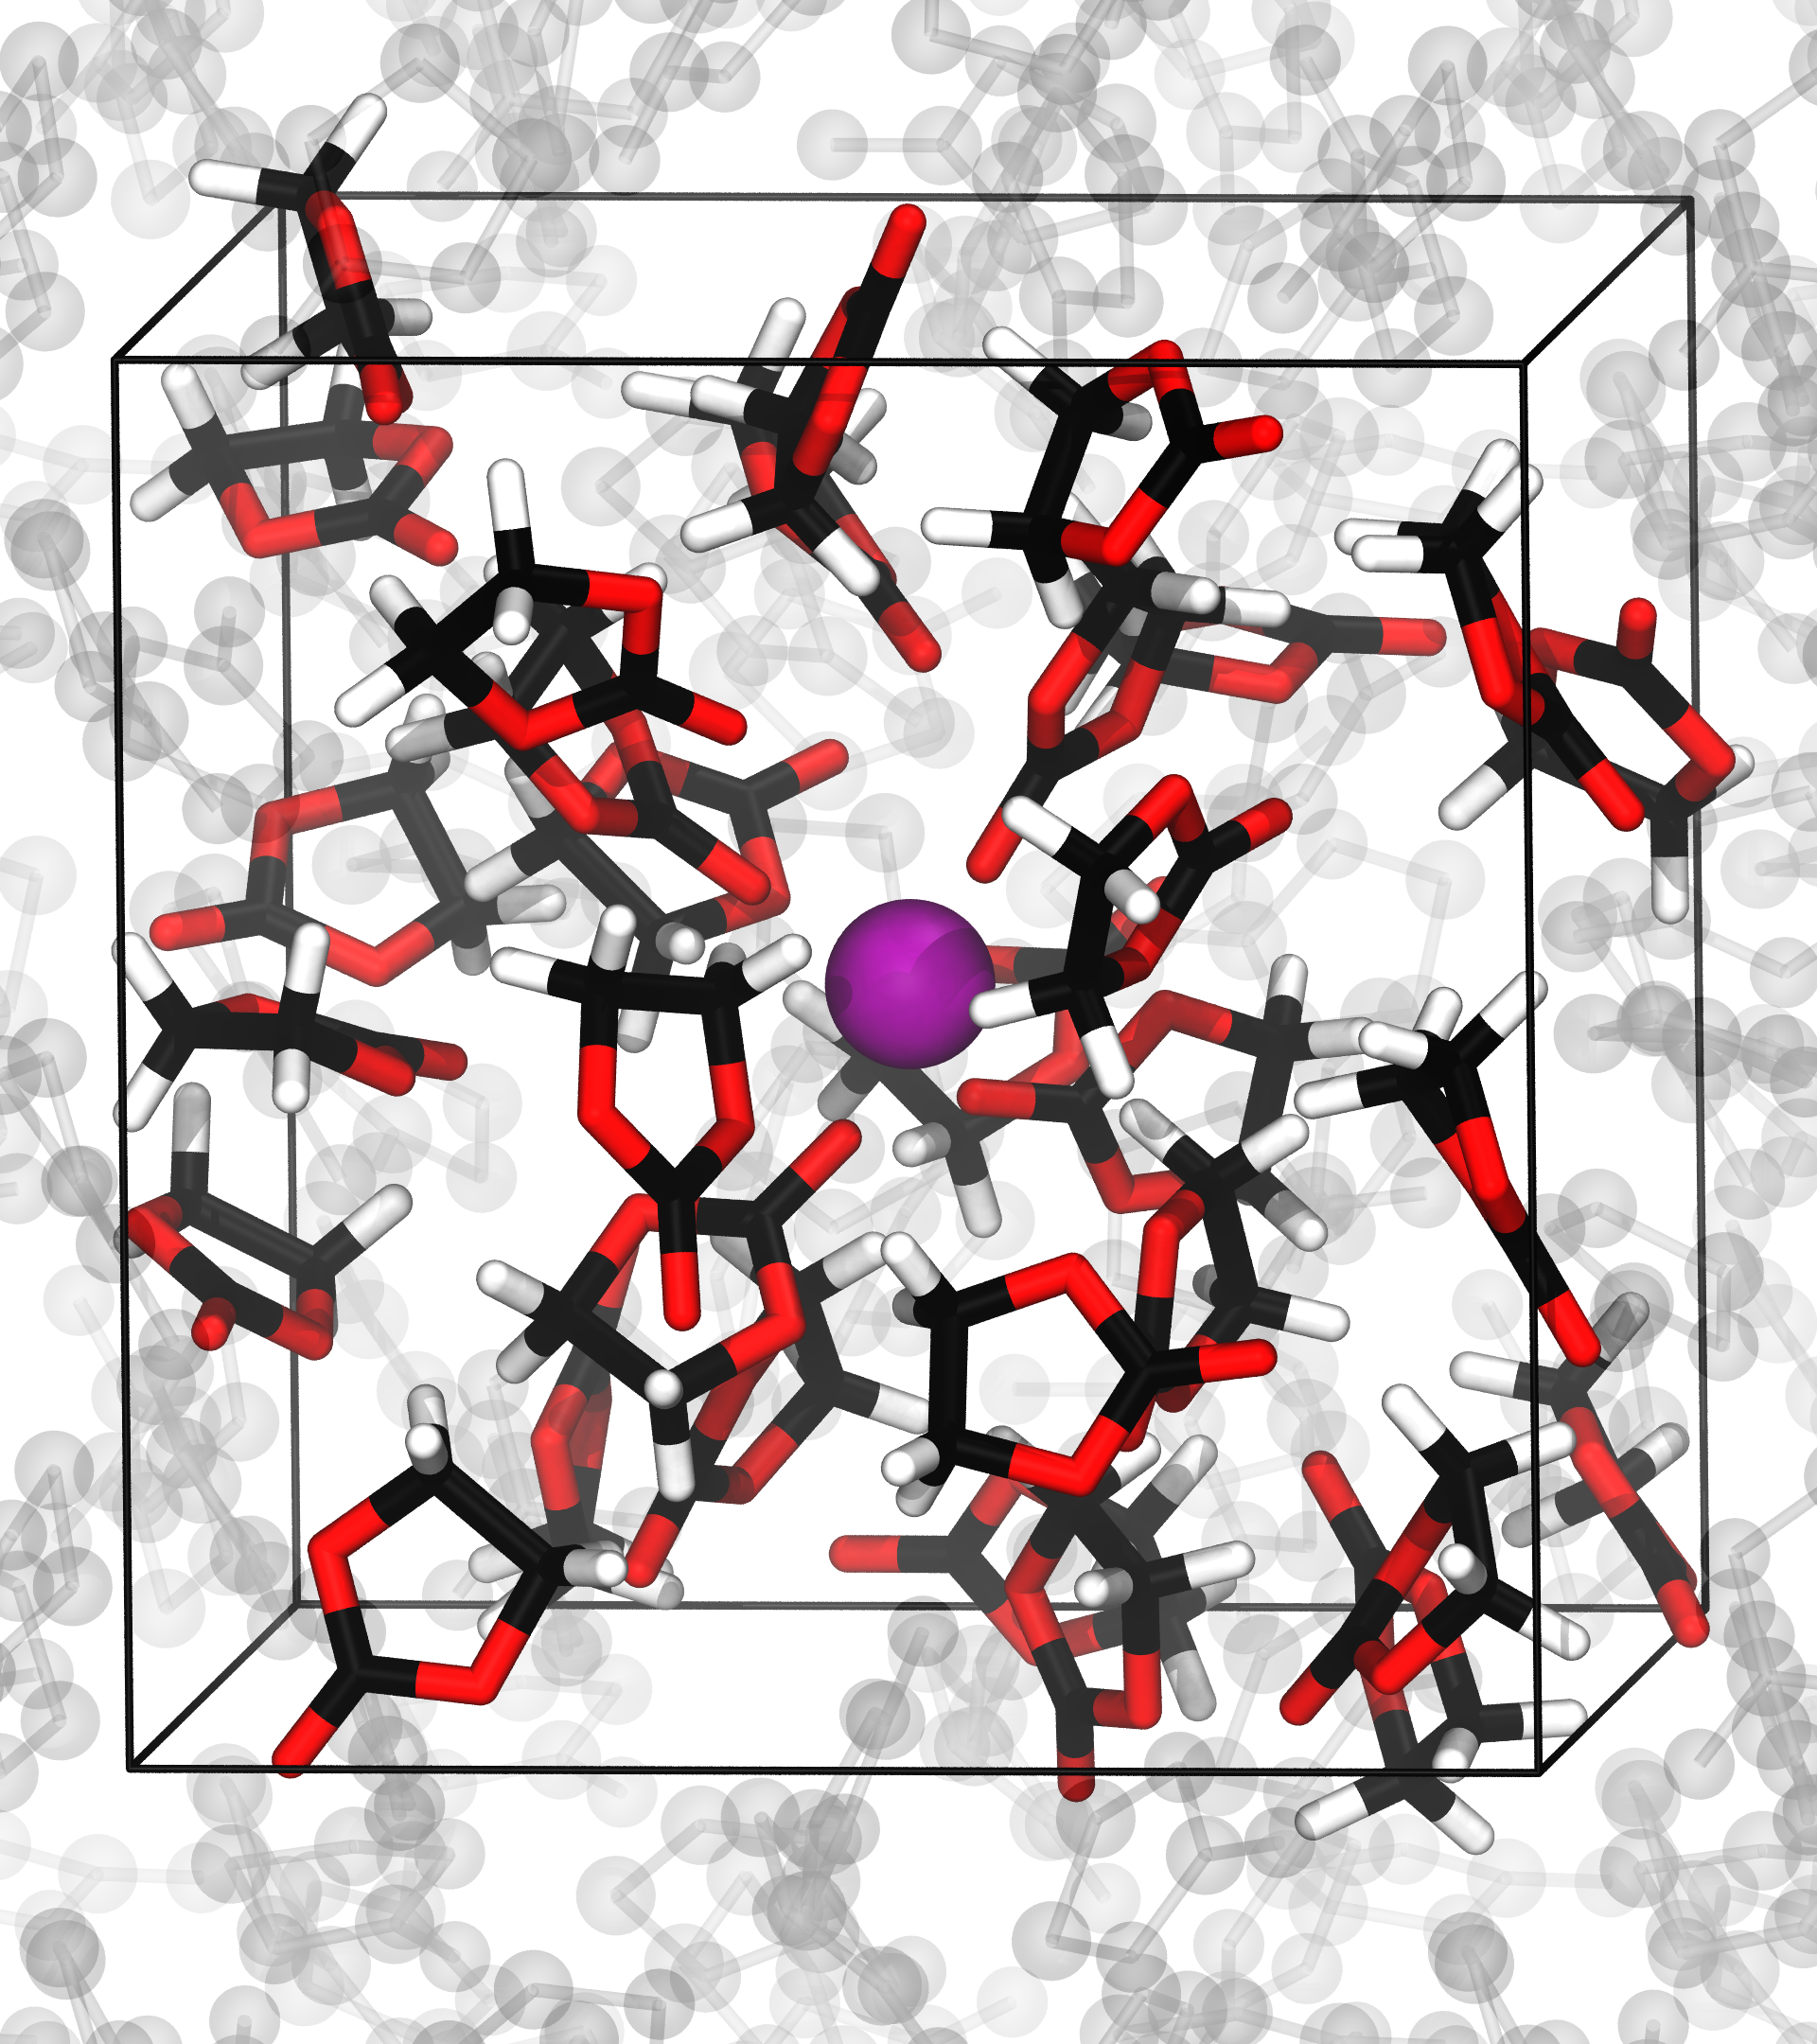
\includegraphics[width=0.98\linewidth]{images/ecpc/toc_liec_default.png}
 \caption[Snapshot of (Li\sur{+}EC\sous{31})]{\label{fig:liec_snap}Snapshot of (Li\sur{+}EC\sous{31}).}
\end{figure}

   \subsection{\label{ch4:sec1:level4}DFT-D3 symmetry adapted perturbation theory}
    Clusters of the nearest 4 molecules centered around the Li\sur{+} ion were extracted from both classical and density functional based trajectories
    of the slightly larger Li\sur{+}EC\sous{31} and Li\sur{+}PC\sous{31} systems. These coordinates were then used as inputs for a symmetry adapted 
    perturbation theory (SAPT) decomposition of the ion/solvent interaction energies at the SAPT(KS)-D3 level. D3 refers to the 3\sur{rd} generation
    dispersion potential of Herbert et al.\cite{lao2014xsaptksd3}. We picked 600 configurations initially, excluding only 2 outliers from the Li\sur{+}EC\sous{31} DFT-generated 
    trajectory and 8 each from the Li\sur{+}PC\sous{31} trajectories for which had produced nonsensical results. We have chosen to retain the the PBE 
    functional in this analysis but slightly increased the accuracy of the basis set to jun-cc-pVDZ and resolution of the identity (RI) approximation 
    optimized jun-cc-pVDZ-RI. Li\sur{+} uses the cc-pVDZ equivalent in both of these basis sets. Benchmarking shows SAPT(KS)-D3 and the related XSAPT 
    method performance is significantly enhanced through the introduction of diffuse functions. The version of SAPT(KS) implemented in QChem 4.4\cite{krylov2013qchem,shao2006qchem} takes 
    advantage of a long-range correction added to the Coulomb potential at a range controlled via a splitting parameter, $\omega$. We optimized the 
    parameters as reported by Herbert et al. with the above basis sets and method\cite{lao2014xsaptksd3}. A value of 8000 bohr\sur{-1} was required for Li\sur{+}, 540 
    bohr\sur{-1} for EC, and 365 bohr\sur{-1} for PC.
  
  \section{\label{ch4:sec2:level1}Results}
   Table \ref{tab:dipoles} lists the average dipole moment of the carbonate molecules from the gas and condensed phase simulations. Error bars were
   calculated with the block-averaging method. A single standard deviation is also included to assess the spread of width the distribution of dipoles.
   Gas phase dipoles for EC exhibited small fluctuations about a mean of 5.44 D. The change from H to CH\sous{3} in PC produced a small increase in 
   the average dipole moment to 5.65 D. In the condensed phase, these dipoles rose by 34\% each! The bulk EC value averaged to 7.30 D and the PC value
   to 7.56 D. Each of these solvents exhibited fluctuations in excess of 0.5 D with EC producing slightly larger fluctuations, possibly owing to the
   more mobile H group and potential steric clashes with neighboring molecules due to the larger CH\sous{3} group. 
   
   Basis set dependence of these quantities is also examined and I found virtually no change in the condensed phase dipoles. There was some 
   fluctuation in the gas phase dipoles just beyond my error estimate, but these settle back down to those predicted by the smallest basis
   set (which I used to generate the trajectories) for the largest basis considered.

\begin{table}
 \begin{center} 
  \begin{tabular}{cccc}
   \hline
   \hline
    System          & $\left<\mu\right>$ & $\sigma$ & $\left<\mu\sous{blk}\right>$/$\left<\mu\sous{gp}\right>$ \\
   \hline
    \\ 
    \multicolumn{4}{c}{\textbf{DZVP-MOLOPT-SR-GTH}} \\ 
    \\
    EC\sous{1,gp}   & 5.44 $\pm$ 0.05   & 0.28 &      \\
    EC\sous{32,blk} & 7.30 $\pm$ 0.22   & 0.55 & 1.34 \\
    PC\sous{1,gp}   & 5.65 $\pm$ 0.07   & 0.29 &      \\
    PC\sous{32,blk} & 7.56 $\pm$ 0.24   & 0.52 & 1.34 \\
    \\ 
    \multicolumn{4}{c}{\textbf{DZVP-MOLOPT-GTH}} \\ 
    \\
    EC\sous{1,gp}   & 5.51 $\pm$ 0.05   & 0.29 &      \\
    EC\sous{32,blk} & 7.30 $\pm$ 0.11   & 0.56 & 1.32 \\
    PC\sous{1,gp}   & 5.71 $\pm$ 0.06   & 0.30 &      \\
    PC\sous{32,blk} & 7.55 $\pm$ 0.14   & 0.53 & 1.32 \\
    \\ 
    \multicolumn{4}{c}{\textbf{TZVP-MOLOPT-GTH}} \\ 
    \\
    EC\sous{1,gp}   & 5.50 $\pm$ 0.05   & 0.29 &      \\
    EC\sous{32,blk} & 7.34 $\pm$ 0.11   & 0.57 & 1.33 \\
    PC\sous{1,gp}   & 5.70 $\pm$ 0.06   & 0.30 &      \\
    PC\sous{32,blk} & 7.59 $\pm$ 0.15   & 0.54 & 1.33 \\
    \\ 
    \multicolumn{4}{c}{\textbf{TZV2P-MOLOPT-GTH}} \\ 
    \\
    EC\sous{1,gp}   & 5.48 $\pm$ 0.05   & 0.29 &      \\
    EC\sous{32,blk} & 7.33 $\pm$ 0.11   & 0.57 & 1.34 \\
    PC\sous{1,gp}   & 5.67 $\pm$ 0.06   & 0.30 &      \\
    PC\sous{32,blk} & 7.58 $\pm$ 0.15   & 0.54 & 1.34 \\
    \\     
    \multicolumn{4}{c}{\textbf{TZV2PX-MOLOPT-GTH}} \\ 
    \\
    EC\sous{1,gp}   & 5.47 $\pm$ 0.05   & 0.29 &      \\
    EC\sous{32,blk} & 7.34 $\pm$ 0.09   & 0.56 & 1.34 \\
    PC\sous{1,gp}   & 5.66 $\pm$ 0.06   & 0.30 &      \\
    PC\sous{32,blk} & 7.58 $\pm$ 0.17   & 0.54 & 1.34 \\    
   \hline
   \hline
  \end{tabular}
  \caption[Gas and condensed phase dipole moments with varying basis set]{\label{tab:dipoles}Dipole moments (in Debye) $\pm$ 
  standard error in the mean using the block averaging method.
  A single sample standard deviation is provided to get a sense of the distribution of molecular dipoles about the mean. 
  The third column is the ratio of the bulk dipole moment to the gas phase measurement.}
 \end{center}
\end{table}

   Solvation structure around the Li\sur{+} ion is shown in Figure \ref{fig:rdf}. Both solvents give peaks in the radial distribution function at a distance of 200 pm.
   The coordination number resulting from integration to the first minimum is about 4 for each solvent. The actual values at the minima are 3.88 at 287.5 pm for EC and 
   3.98 at 277.5 pm for PC. The cutoff is very clean for PC and less so for EC where the g(r) smoothly increases through to the second, much broader shell which peaks 
   in both solvents just shy of 800 pm.

\begin{figure}
 \begin{center}
 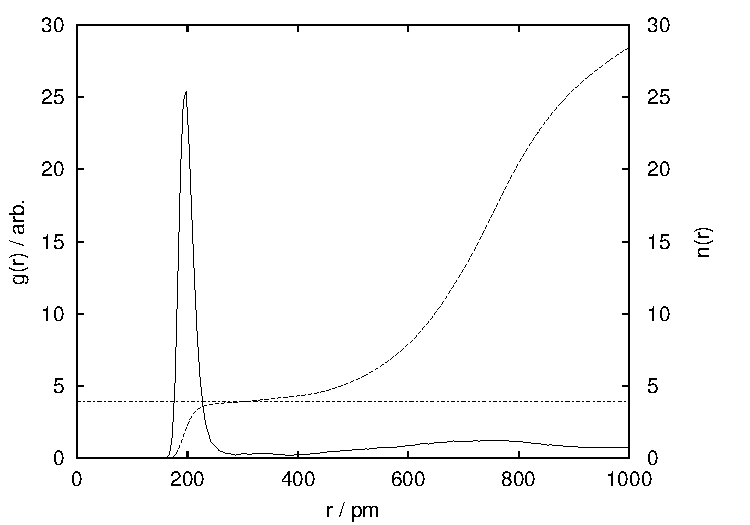
\includegraphics[width=0.8\linewidth]{images/ecpc/liec_32-noWC-rdf.pdf} \\
 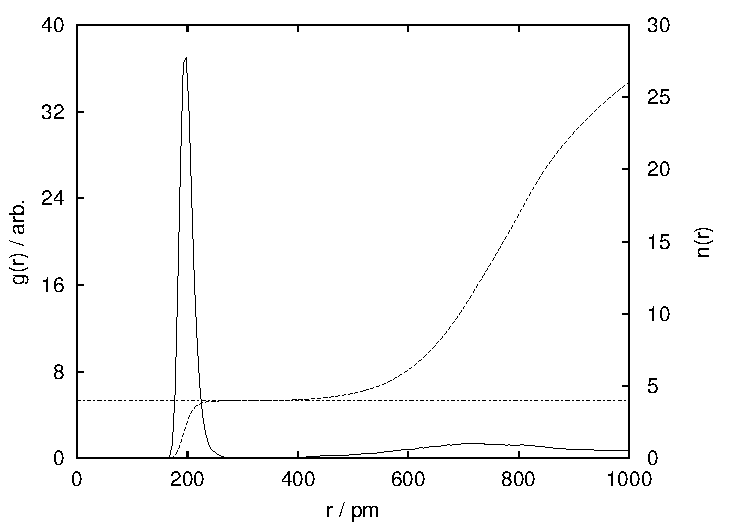
\includegraphics[width=0.8\linewidth]{images/ecpc/lipc_32-noWC-rdf.pdf}
 \end{center}
 \caption[Li$^{+}$ and carbonyl oxygen radial distribution functions]{\label{fig:rdf}Li\sur{+} and carbonyl oxygen radial distribution 
 functions for ethylene carbonate (top) and
 propylene carbonate (bottom). The distribution function is depicted with a solid line while the number integral is 
 shown as a dashed line. A dashed horizontal line passes provides an estimate of the coordination number in the first
 solvation shell which are both very close to n $=$ 4.}
\end{figure}

   The distribution of dipole moments of EC and PC molecules as a function of distance from the Li\sur{+} are shown in Figures \ref{fig:ec_cdf} and \ref{fig:pc_cdf}. 
   Horizontal lines in these plots point out the gas phase and condensed phase averages from above (from the DZVP-MOLOPT-SR-GTH data). These dipoles are also computed 
   with the short range basis. The x-axis reflects the distance between the ion and carbonyl oxygen. The density distribution of the EC molecules maxes near the ion
   at a dipole moment of $\sim$8.4--8.5 D and in PC at $\sim$8.7--8.8 D. Each of these figures is slightly greater than 50\% larger than those measured in the gas 
   phase and approaching 20\% larger than those measured in neat solutions. The wide spread of the dipole moments in the first shell is indicative of the fairly 
   labile nature of the solvation shell for EC especially. There's definitely more accumulation between the first and second solvation shells for this system which
   corresponds to the solvent in reverse orientation with the carbonyl directed away from the ion. This appeared to occur less frequently in PC, probably because 
   PC is modeled at a lower temperature.

\begin{figure}
 \begin{center}
 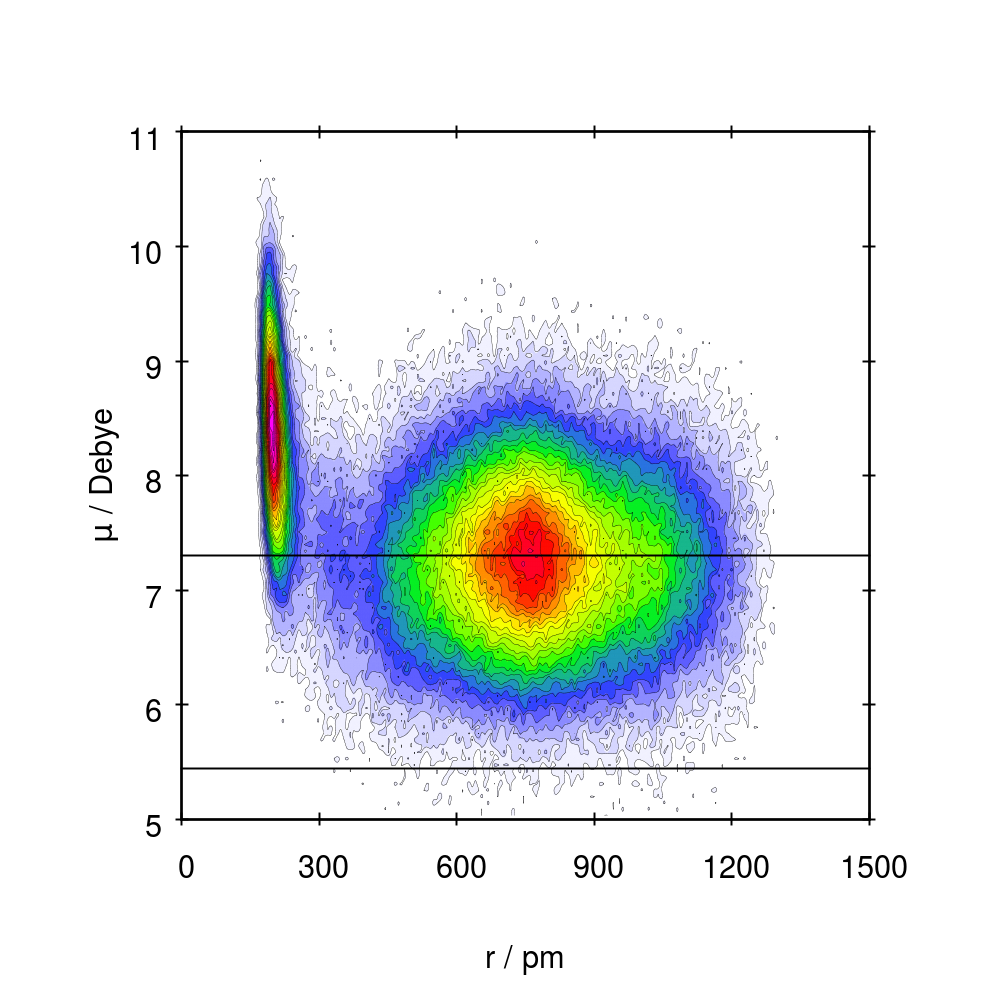
\includegraphics[width=0.98\linewidth]{images/ecpc/cdf_2_rdf_dipoleC3H4O3.png} \\
 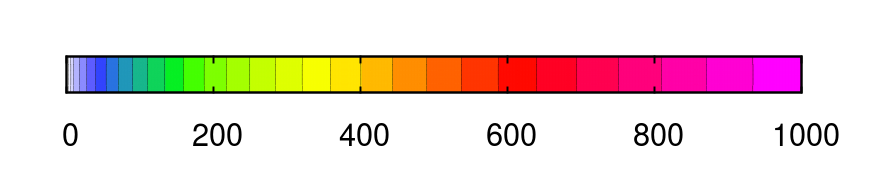
\includegraphics[width=0.5\linewidth]{images/ecpc/cdf_2_rdf_dipoleC3H4O3_box.png}
 \end{center} 
 \caption[Ethylene carbonate dipoles versus distance from ion]{\label{fig:ec_cdf}Combined density distribution of ethylene 
 carbonate dipole moment as a function of radial
 distance from the ion. Colors map to raw counts delineated in the color bar. Solid, horizontal lines highlight average
 gas and condensed phase dipole moments from Table \ref{tab:dipoles}. Images aren't centered because I will be adding an 
 image to the upper right corner.}
\end{figure}

\begin{figure}
 \begin{center}
 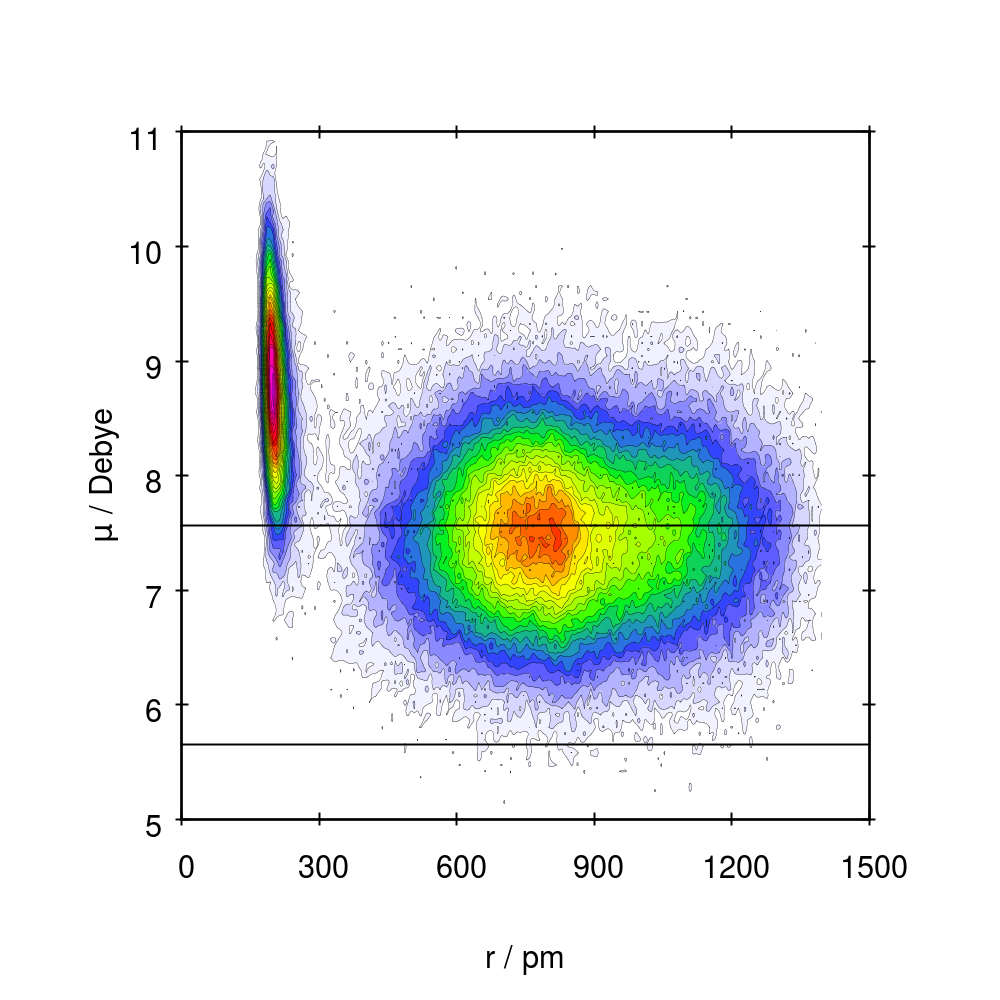
\includegraphics[width=0.98\linewidth]{images/ecpc/cdf_2_rdf_dipoleC4H6O3.png} \\
 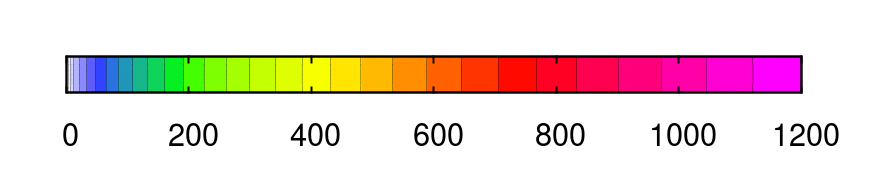
\includegraphics[width=0.5\linewidth]{images/ecpc/cdf_2_rdf_dipoleC4H6O3_box.png}
 \end{center} 
 \caption[Propylene carbonate dipoles versus distance from ion]{\label{fig:pc_cdf}Combined density distribution of propylene
 carbonate dipole moment as a function of radial
 distance from the ion. Colors map to raw counts delineated in the color bar. Solid, horizontal lines highlight average
 gas and condensed phase dipole moments from Table \ref{tab:dipoles}. Image not centered, same reason.}
\end{figure}

   SAPT(KS)-D3 results are shown in Figures \ref{fig:ecsapt1} through \ref{fig:pcsaptint}. The more rigid nature of the classical force field universally produced
   less broad distributions in the energy terms than the density-functional configurations. The greater bond length between the ion and solvent in the GAFF model
   likewise produced smaller attractive energies, though the disparity is greater for PC configurations than EC. This also produced less overlap between the atoms
   and so gave smaller exchange and exchange-coupled energy contributions. For EC, the greatest differences were reflected in the induction energies. In PC, both
   1\sur{st} and 2\sur{nd} order energy contributions failed to overlap significantly. In the total intermolecular energies (which include dispersion and the infinite
   order corrections), there is greater overlap between the classical and \emph{ab initio} models with EC and very little for PC. These data suggest that the force 
   field relies on error cancellation (the smaller exchange energies) to make up for their underestimation of attractive components due to the longer bond lengths.

  \section{\label{ch4:sec3:level1}Discussion}
   The dipole moments I report are a fair bit larger than those often used in literature. For pure EC and PC, 4.61 D and 4.81 D are most often cited\cite{ayse2016ecpc,peruzzi2015solvation}.
   These are each about 85\% of the values reported in Table \ref{tab:dipoles}. However, the larger dipole moments found here match those from the theoretical predictions of Hammer et 
   al.\cite{hammer2004dipole}, Luber\cite{luber2014local} (including the condensed phase $\left<\mu\right>$ and standard deviation for EC), Masia et al.\cite{masia2004ethylene}, Park et 
   al.\cite{park2011low}, Stark-effect measurements by Alonso et al.\cite{alonso1986microwave}, and back-calculating the dipole from capacitance measurements by Chernyak\cite{chernyak2006dielectric}. 
   Only the works of Park et al. and Chernyak made an attempt at the dipole moment of PC. Chernyak's estimate of the EC dipole is 4.81 D but 5.36 D for PC, closer to the result I 
   obtained\cite{chernyak2006dielectric}.
   
   Interaction energies are an interesting story as well. Averages taken of my data in Figures \ref{fig:ecsaptint} and \ref{fig:pcsaptint} are nearly identical, though the EC distribution
   is obviously a fair bit broader than the PC one. This reflects the increased frequency of structures where one of the solvent molecules is being exchanged with the bulk and is often
   nearly completely turned around. This is seen in Figures \ref{fig:ec_cdf} and \ref{fig:pc_cdf} as the increased density of ion-carbonyl oxygen distances around 300 pm. Given that an
   increased temperature in the Li\sur{+}/PC simulations would serve to broaden the interaction energy distribution and that the largest binding energies were observed for Li\sur{+}/EC 
   despite the greater thermal stresses, it is reasonable to conclude that the binding energy between Li\sur{+}/EC is greater than Li\sur{+}/PC, consistent with some of the experiments 
   discussed in Chapter \ref{ch1:sec5:level1}. However, Peruzzi et al. found the solvation enthalpies of KX salts were more favorable in PC than EC. The binding energies of Park et al.
   support this conclusion as well\cite{park2011low}, as does the SAPT work by Arslanargin et al.\cite{ayse2016ecpc}. There's a split in the thermodynamic data of anions at Cl\sur{-}
   which was determined to be better solvated in EC than PC. The similar solvent reorganization energies in this study suggest that the differences lie primarily in the strength of 
   ion/solvent interactions. My SAPT energies using classically generated coordinates favor Li\sur{+}/EC over Li\sur{+}/PC while K\sur{+} was found to be better solvated in PC\cite{ayse2016ecpc}. 
   There may be a cutoff here as well, similar to that in water. Clearly, there is no consensus on relative binding energies of ions with the cyclic carbonates.
   
   Radial distribution functions and the coordination number have been another point of contention in the literature. As reviewed earlier in Chapter \ref{ch1:sec5:level1}, the 
   coordination number is typically taken to be somewhere in the range of 4--5, though it has been determined to be as high as $\sim$7\cite{castriota2003temperature}. The integral
   taken to the minimum of the first peak of my radial distribution functions in Figures \ref{fig:rdf} is $\sim$4 in each solvent. Again, the actual values were found to be 3.88 for EC 
   and 3.98 for PC. These values are identical to those from other theoretical studies but smaller than most of the experimental measurements discussed previously. Since the methodology
   I used was based off of the work of Leung et al.\cite{leung2010liion}, it's excellent to see that our g(r) have very similar profiles. Both g(r)'s peak at 200 pm for the Li\sur{+}-O(carbonyl) distance
   and have an intensity of just over 25. Distributions taken from Arslanargin et al.\cite{ayse2016ecpc} and Masia et al.\cite{masia2004ethylene} show over-structuring of the first 
   solvation shell, each with intensities over 40. The location of the maximum in each of these distributions also differs from both mine and Leung's. The classical models tend to give
   too small an average bond length between Li\sur{+} and EC, though one of the results from Arslanargin et al.\cite{ayse2016ecpc} gives too great a distance (and a coordination number
   of 6). This model is identical to the one used in this study to prepare the initial coordinates for AIMD work. For PC, the location of the first peak was found by Smith et al.\cite{smith2014x} 
   to also be around 200 pm, though their simulated model is less structured than mine with an intensity similar to that of my Li\sur{+}/EC result. This may simply reflect temperature 
   differences.

  \section{\label{ch4:sec4:level1}Conclusions $\&$ Future Work}
   Up to this point, I have determined that polarizability is an important consideration in the condensed phase behavior of cyclic carbonates ethylene carbonate and propylene carbonate.
   The dipole moments which were found to be 5.44 D and 5.65 D in the gas phase increase by $\sim$34\% through self-polarization in the condensed phase to 7.30 D and 7.56 for EC and PC,
   respectively. This increase may be approximately handled in classical models which appear to reproduce the dielectric constant of the pure solvents over a broad temperature range\cite{you2015dielectric}.
   However, when attempting to address problems of ion solvation, the dipole moments of these solvents increase even further by about 50\% over the gas phase dipole moments to about
   $\sim$8.4--8.5 D and in PC at $\sim$8.7--8.8 D in the first solvation shell around Li\sur{+}. While in water there is some evidence to suggest that the dipole moments of waters
   coordinated to the ions more or less return to the bulk value or produce modest increases ($<$10\%)\cite{heuft2003cl,heuft2005f,heuft2005i,krekeler2006density,lightstone2001first}, it is clear from my results that this may not be the case 
   in solvents with larger polarizabilities. Interaction energies suggested better solvation of Li\sur{+} in EC than in PC, though the extent to which EC is favored cannot be predicted
   from these results. The coordination structure of EC and PC around Li\sur{+} compared well against other simulation results and the coordination numbers were found to be very close 
   to 4 in each of the solvents, consistent with other theoretical calculations. These fall short of the assumed values from experimental measurements which tend closer to 5 EC or PC
   per Li\sur{+}.
   
   Before publishing this work I have several other pieces of data to add and I may collaborate with Matthew Brown to calculate X-ray absorption spectra to predict Li\sur{+}-1s binding
   energies. The binding energy of the core state was shown by Matt Brown to be a probe of the strength of ion/solvent interactions\cite{brown2015ion}. By comparing the binding energy
   in a fictitious state where the gas phase optimized EC and PC molecules are superimposed on the positions of solvent molecules in Li\sur{+}/XC\sous{4} clusters (X = E and P) versus 
   the binding energy of the Li-core state in the fully interacting cluster, I hope to approximately determine the effect of polarization. Alternative approaches will likely be 
   considered as well. Another possibility is to perform a many-body expansion where a distinguished EC or PC interaction energy is measured with Li\sur{+} left out.
   I am also going to add data for PC simulated at 450 K as well. The choice of 350 K was motivated to mimic the temperature increase in EC over its melting point 
   to simulate a liquid phase just above each solvent's freezing temperature. It is clear that a 450 K simulation of PC would prove useful in addressing some other concerns about the
   binding energy and X-ray spectra by eliminating the thermal differences. The additional data includes sampling the dipole moments from the simulations using the GAFF model, calculating 
   interaction energies for small clusters using the GAFF interaction potential, and measuring EC and PC structural properties of molecules in the first shell and relating them to their
   dipole moment (to address how the structure changes to produce the larger dipole moment).
  
\end{ecpc}
